% !TEX encoding = UTF-8 Unicode
%% LyX 2.1.4 created this file.  For more info, see http://www.lyx.org/.

%%%%%%                                              PREAMBULE                                        %%%%%%%%%%%%%%

%%%%%%%%%% LisezMoi
% Le rapport LaTex est muni de 2 fonctions très pratiques:
%   	-image : affiche une image rangée dans le dossier /figures, bien  % centrée, avec une légende et tout
%   	-imageb : la même chose, mais gère deux images côte à côte

% Ca marche comme ça:

% \image{width = 15cm}{nom}{légende}
% \imageb{nom1}{l\'egende1}{nom2}{légende2}

% rajoutez vous en auteur quand vous éditez
%%%%%%%%%%

\documentclass[12pt,french]{report}
\usepackage[T1]{fontenc}
\usepackage[utf8]{inputenc}
\usepackage[a4paper]{geometry}
%\usepackage{vmargin}
%\setmarginsrb{3cm}{0.5cm}{3cm}{2.0cm}{1,5cm}{0.5cm}{1.0cm}{2.0cm}

\makeatletter

%% User specified LaTeX commands.
\usepackage{graphicx,graphics,color}
%\usepackage{multirow}
\usepackage{transparent}
\usepackage{eso-pic}
\usepackage{url}
\usepackage{cite}

\usepackage{color}
\usepackage{listings}
\usepackage{setspace}

\usepackage{float}

\definecolor{Code}{rgb}{0,0,0}
\definecolor{Decorators}{rgb}{0.5,0.5,0.5}
\definecolor{Numbers}{rgb}{0.5,0,0}
\definecolor{MatchingBrackets}{rgb}{0.25,0.5,0.5}
\definecolor{Keywords}{rgb}{0,0,1}
\definecolor{self}{rgb}{0,0,0}
\definecolor{Strings}{rgb}{0,0.63,0}
\definecolor{Comments}{rgb}{0,0.63,1}
\definecolor{Backquotes}{rgb}{0,0,0}
\definecolor{Classname}{rgb}{0,0,0}
\definecolor{FunctionName}{rgb}{0,0,0}
\definecolor{Operators}{rgb}{0,0,0}
\definecolor{Background}{rgb}{0.98,0.98,0.98}
\lstdefinelanguage{Python}{
numbers=left,
numberstyle=\footnotesize,
numbersep=1em,
xleftmargin=1em,
framextopmargin=2em,
framexbottommargin=2em,
showspaces=false,
showtabs=false,
showstringspaces=false,
frame=l,
tabsize=4,
% Basic
basicstyle=\ttfamily\small\setstretch{1},
backgroundcolor=\color{Background},
% Comments
commentstyle=\color{Comments}\slshape,
% Strings
stringstyle=\color{Strings},
morecomment=[s][\color{Strings}]{"""}{"""},
morecomment=[s][\color{Strings}]{'''}{'''},
% keywords
morekeywords={import,from,class,def,for,while,if,is,in,elif,else,not,and,or,print,break,continue,return,True,False,None,access,as,,del,except,exec,finally,global,import,lambda,pass,print,raise,try,assert},
keywordstyle={\color{Keywords}\bfseries},
% additional keywords
morekeywords={[2]@invariant,pylab,numpy,np,scipy},
keywordstyle={[2]\color{Decorators}\slshape},
emph={self},
emphstyle={\color{self}\slshape},
%
}
\lstset{language=Python}


\newcommand{\image}[3]{% 1: param image> latex( height=5cm, width...) 2: nom_fic / 3: legend
	\begin{figure}[h]%
	\begin{center}%
	\includegraphics[#1]{figures/#2}%
	\end{center}
	\caption{#3}
	\label{#2}
	\end{figure}
}

\newcommand{\imageb}[4]{%
	\begin{figure}
	\begin{minipage}[t]{.47\linewidth}
	\begin{center}%
	\includegraphics[width= \textwidth]{figures/#1}
	\caption{#2}\label{#1}%
	\end{center}%
	\end{minipage}
	\hfill
	\begin{minipage}[t]{.47\linewidth}
	\begin{center}%
	\includegraphics[width= \textwidth]{figures/#3}
	\caption{#4}\label{#3}%
	\end{center}%
	 \end{minipage}
	\end{figure}
}

\newcommand{\refp}[1]{
	\ref{#1}, page \pageref{#1}
}


\newcommand\BackgroundPic{%
	\put(0,0){%
	\parbox[b][\paperheight]{\paperwidth}{%
	\vfill
	\centering
	{\transparent{0.4} \includegraphics[width=18cm,height=\paperheight,%	
	keepaspectratio]{figures/background}}%
	\vfill
}}}


%\setcounter{page}{4}

\AtBeginDocument{
  \def\labelitemi{\(\triangleright\)}
}

\makeatother

\usepackage[french]{babel}
\makeatletter

\addto\extrasfrench{%
   \providecommand{\og}{\leavevmode\flqq~}%
   \providecommand{\fg}{\ifdim\lastskip>\z@\unskip\fi~\frqq}%
}

\makeatother


%----------------------------------------------------------------------------------------
%	TITLE PAGE
%----------------------------------------------------------------------------------------

\newcommand*{\titleGP}{\begingroup % Create the command for including the title page in the document
\centering % Center all text
\vspace*{\baselineskip} % White space at the top of the page


PROJET DATA 
\rule{\textwidth}{1.6pt}\vspace*{-\baselineskip}\vspace*{2pt} % Thick horizontal line
\rule{\textwidth}{0.4pt}\\[\baselineskip] % Thin horizontal line

{\LARGE Data Challenge Reminiz : Reconnaissance de célébrités}\\[0.2\baselineskip] % Title

\rule{\textwidth}{0.4pt}\vspace*{-\baselineskip}\vspace{3.2pt} % Thin horizontal line
\rule{\textwidth}{1.6pt}\\[\baselineskip] % Thick horizontal line

\scshape % Small caps
2017--2018\par % Location and year

\vspace*{2\baselineskip} % Whitespace between location/year and editors

{Daviet Mathieu\\
Hélénon François\\
Yan Sen\\\par} % Editor list
\vspace*{2\baselineskip} % Whitespace between location/year and editors
{\itshape \par} % Editor affiliation

\vspace*{6\baselineskip} % Whitespace between location/year and editors

\begin{flushleft} \large
\emph{Superviseurs}\\
Pennerath Frédéric \\
\end{flushleft}

\vfill % Whitespace between editor names and publisher logo

\includegraphics[width=5cm]{image_rapport/logo.jpg}

{\scshape 2018} \\[0.3\baselineskip] % Year published
%{\large THE PUBLISHER}\par % Publisher

\endgroup}



%%%%%%%%%%%%%%%%%  DEBUT DU RAPPORT  %%%%%%%%%%%%%%%%%%%%%%%%%%%%

\begin{document}

\titleGP

\clearpage


%\renewcommand{\chaptername}{Partie}
%\renewcommand{\partname}{Séquence}
\thispagestyle{empty}
\newpage{}

\tableofcontents
\clearpage

\chapter{Présentation Challenge Reminiz}

\section{Contexte}
Reminiz cherche à identifier en temps réels des personnages publiques à la télévisons  (acteurs, chanteurs, présentateurs tv...). Un utilisateur pourrait ainsi filtrer le contenu en fonction d ses acteurs préférés à des fins ludiques ou de recherches documentaires.
Dans cette optique il cherche des algorithmes qui puissent être à la fois précis et permettre un traitement rapide afin  de pouvoir traiter la quantité considérable de contenu vidéo existante.

\section{Objectifs spécifiques du challenge}

Le but du challenge est de reconnaître un certain nombre de célébrités apparaissant dans une ou plusieurs sources vidéos différentes.

La mesure d'évaluation est tout simplement le taux  de classification correcte.

\subsection{Base de données}

On dispose d'un set d'entraînement composé de:

\begin{itemize}
	\item 9888 images téléchargées sur internet correspondant à 992 acteurs différents ainsi qu'une classe anonyme. Il y a environ une dizaine de d'image par classes (1 acteur = 1 classe)
	\item 97442 images groupées en 2461 tracks. Un track est une séquence de quelques images extraites d'une scène d'un film ou d'un épisode de série. Les images sont donc très proches les unes des autres. Un track contient en général un seul acteur (voir figure  \ref{"track"}). Chaque track contient un identifiant unique renseignant sur le film dont le track est issu.
\end{itemize}


Les images internets et les celles extraites dans les tracks sont annotées avec un identifiant unique par acteur.

On dispose également d'un set de tests composé de:
\begin{itemize}
	\item 25989 images groupées en 677 tracks. Les identifiants des track suivent la même nomenclature que pour le set d'entraînement ce qui renseigne sur le film dont sont issus les tracks. 
	\item Pas d'images de type "internet"
\end{itemize}


Les images sont de tailles et de qualités variables que ce soit pour les tracks ou les images internets.

\begin{figure}[h]
	\begin{minipage}[t]{.47\linewidth}
		\begin{center}%
			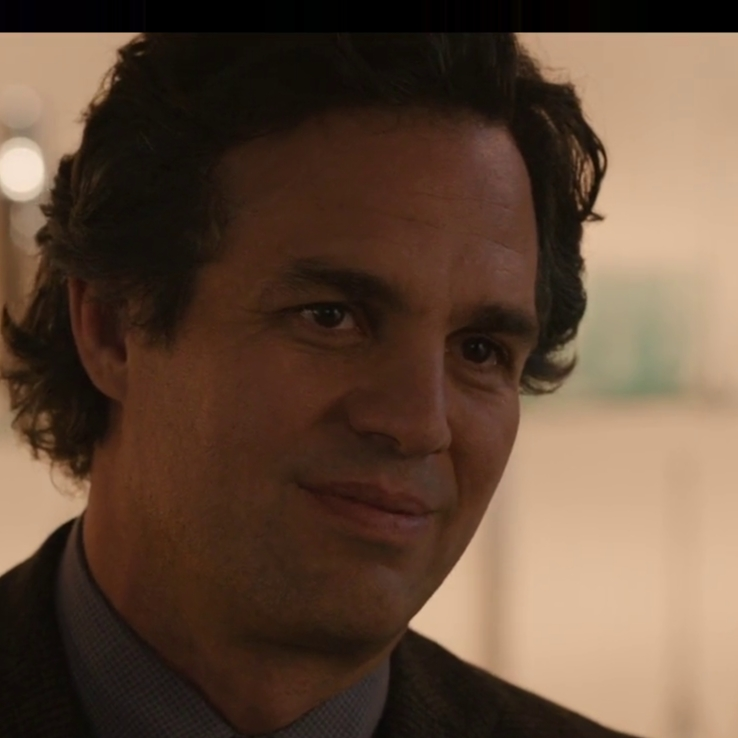
\includegraphics[width= \textwidth]{image_rapport/275.jpg}
		\end{center}%
	\end{minipage}
	\hfill
	\begin{minipage}[t]{.47\linewidth}
		\begin{center}%
			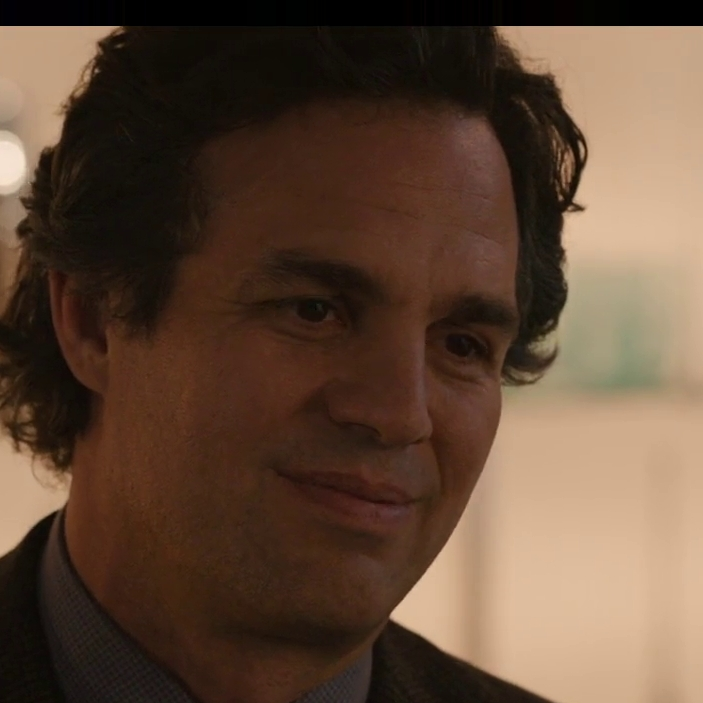
\includegraphics[width= \textwidth]{image_rapport/277.jpg}
		\end{center}%
	\end{minipage}
	\caption{Exemple de 2 images issues d'un même track}\label{"track"}%
\end{figure}

\chapter{Classification par réseau neuronal profond}

\section{Exploitation base de données}
Une première étape importante est de pouvoir manipuler les bases de tests et d'entraînement.
Charger et travailler sur toutes la base de données en une fois est impossible car la mémoire vive est très vite saturée. Il a fallu charger intelligemment les images par batchs de données et stocker des résultats intermédiaires sur disque afin de pouvoir faire tous les traitements décrits dans la suite du rapport.

Par ailleurs afin d'accélérer les traitements, on utilise les fonctionnalités de multiprocessing de python afin de réaliser en parallèle le chargement en mémoire et le prétraitement des images (voir figure \ref{"pipeline"}).


\begin{figure}[H]
		\begin{center}%
			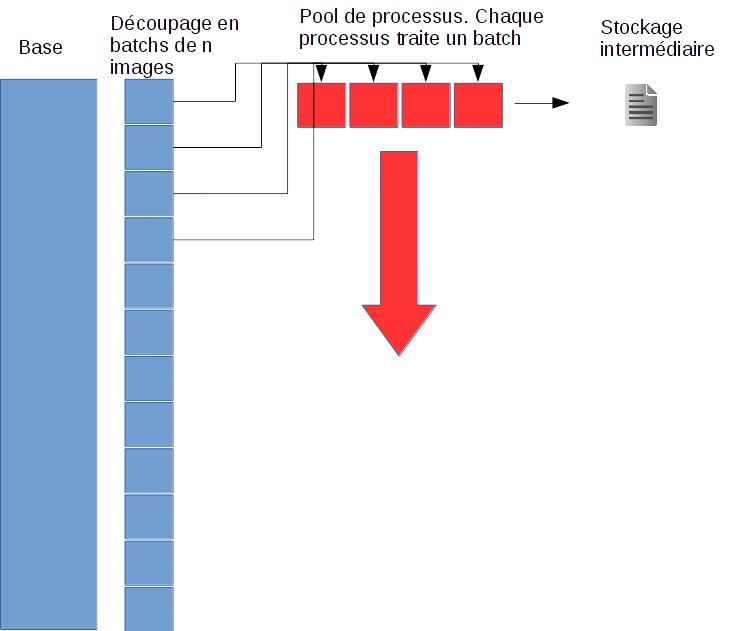
\includegraphics[scale=0.5]{image_rapport/pipeline.jpg}
		\end{center}%
	\caption{Procédure de traitement des images}\label{"pipeline"}%
\end{figure}



\section{Un réseau pré-entrainé le Vgg-Face}
Les réseaux convolutions profonds ont montré de très bonnes performances ces dernières années dans la reconnaissance d'objets et de personnes. L'apprentissage de tel réseaux pouvant demander des jours voire semaines de calcul sur des plateformes performantes, plutôt que de chercher à créer notre propre réseau, nous avons utilisé un réseau pré-entrainé. 
Une équipe d'Oxford \cite{vgg} a notamment entraîné un réseau pour la classification de visages sur des personnalités et des bases de données différentes de celles utilisées par Reminiz.

Les couches "cachées" d'un réseau profond extraient des caractéristiques complexes des signaux d'entrées tandis que les dernières couches se chargent de la classification.

L'idée est alors que les couches cachées ont pu apprendre à extraire des caractéristiques suffisamment robustes et généralisables pour l'appliquer à notre cas.

On a alors téléchargé les poids du réseau et on les a utilisés après avoir recréer l'architecture du vgg-face sous le framework Keras.
On a supprimé les dernières couches du réseau responsables de la classification.

Finalement on obtient en sortie du réseau un vecteur de 2622 features supposées représentatifs d'un visage.

\section{Problèmatiques spécifiques à Reminiz}
On peut cependant soulever certains problèmes liés à l'utilisation d'un réseau pré-entrainé.
L'apprentissage a été réalisée sur des sets d'images  particuliers et il faut donc adapter notre base de données pour que les images correspondent au même "type" d'image utilisée pour l'apprentissage du réseau.
On peut notamment penser aux différences suivantes entre les images issues des bases du Vgg et celles des séquences de films :
\begin{itemize}
	\item Images de taille 224*224*3 vs taille  variable
	\item Personnalités de face, visage vertical vs orientation diverses des visages
	\item Images ne contenant que le visage (pas le corps) vs images contenant le haut du corps
	\item Bonne condition d’éclairage en générale vs éclairage variable

\end{itemize}

Afin de maximiser la reconnaissance il est donc nécessaire de pré-traiter les images.


\begin{figure}[H]
	\begin{minipage}[b]{.47\linewidth}
		\begin{center}%
			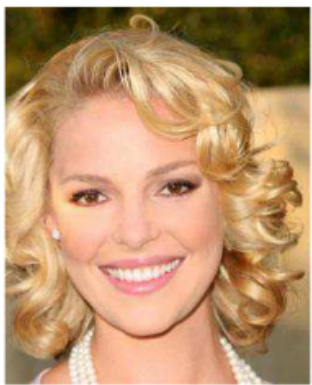
\includegraphics[width= 224px,height=224px]{image_rapport/v4.png}
		\end{center}%
	\end{minipage}
	\hfill
	\begin{minipage}[b]{.47\linewidth}
		\begin{center}%
			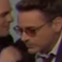
\includegraphics{image_rapport/v3.png}
		\end{center}%
	\end{minipage}
	\caption{Comparaison d'une image issue des bases du vgg à gauche vs celle issues d'une séquence de film à droite}\label{"com"}%
\end{figure}

\chapter{Prétraitement des images}
Dans ce chapitre, on va essayer de améliorer les données. On les réaliser par 2 étapes: détecter le visage et tourner le visage afin d'assurer que le visage est au centre de l'image.

\section{Détection de visage}
Afin de détecter le visage, il existe beaucoup de méthodes : HOG (\emph{histogramme de gradient orienté}), le descripteur de Haar, réseau neuronal profond...

Dans notre premier essai, on applique HOG. On trouve que la boîte de délimitation du visage n'est pas très précise et qu'il existe le cas que quelques visages ne peuvent pas être détectés.

Dans notre deuxième essai, on applique le descripteur de Haar. On trouve que la boîte de délimitation du visage est plus précis que celui de HOG, mais qu'il y a plus de visages qui ne sont pas détectés dans la base de données (voir figure \ref{"haar"}). De plus, sî une image contient un visage avec son ombre, le descripteur de Haar va reconnaître l'ombre comme un visage (voir figure \ref{"ombre"}).
\begin{figure}[H]
    \begin{center}%
		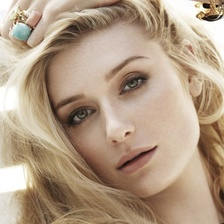
\includegraphics[scale=0.5]{image_rapport/09.jpg}
		\end{center}%
	\caption{le visage peut être détecté par HOG, mais ne peut pas être détecté par le descripteur de Haar }\label{"haar"}%
\end{figure}

\begin{figure}[H]
    \begin{center}%
		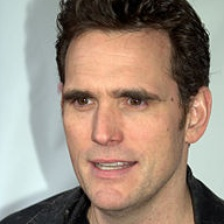
\includegraphics[scale=0.5]{image_rapport/05.jpg}
		\end{center}%
	\caption{un visage avec son ombre}\label{"ombre"}%
\end{figure}

Afin d'éviter les imperfections des méthodes précédantes, on utilise un modèle déjà entraîné dans le librairie \emph{Dlib} à détecter les 68 repères de vissage (voir figure \ref{"landmarks"}). On trouve qu'il y a très peu de visages ne peuvent pas être détectés.

\begin{figure}[H]
    \begin{center}%
		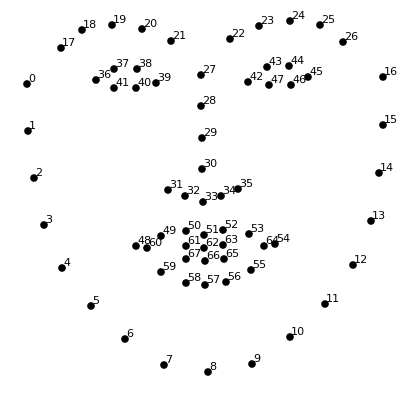
\includegraphics[scale=0.5]{image_rapport/landmarks.png}
		\end{center}%
	\caption{un visage avec son ombre}\label{"landmarks"}%
\end{figure}

\section{Transformation affine }
Etant donné les visages détectés, on va faire la transformation affine afin d'assurer les visages sont au centre des images. On va trouver les repères des yeux et tourner l'image pour assurer les yeux sont dans le sens horizontal (voir figure \ref{"prj"}).

\begin{figure}[H]
	\begin{minipage}[b]{.47\linewidth}
		\begin{center}%
			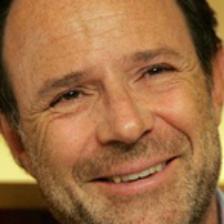
\includegraphics{image_rapport/img2.png}
		\end{center}%
	\end{minipage}
	\hfill
	\begin{minipage}[b]{.47\linewidth}
		\begin{center}%
			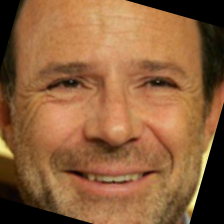
\includegraphics{image_rapport/img2b.png}
		\end{center}%
	\end{minipage}
	\caption{transformation affine}\label{"prj"}%
\end{figure}


\bibliographystyle{plain}
\bibliography{biblio}

\end{document}